\documentclass[tikz,border=10pt]{standalone}
\usepackage{amsmath}
\usetikzlibrary{arrows.meta, positioning, calc, fit, decorations.pathreplacing}

\definecolor{c1}{HTML}{000000}  % black       - structure, axes
\definecolor{c2}{HTML}{233D4D}  % deep slate  - the windows we impose
\definecolor{c3}{HTML}{FE7F2D}  % orange      - the measurements themselves
\definecolor{c4}{HTML}{EAECF0}  % cool grey   - panel fills
\definecolor{axiscolor}{HTML}{333333}
\definecolor{labelcolor}{HTML}{5F6B75}

\begin{document}
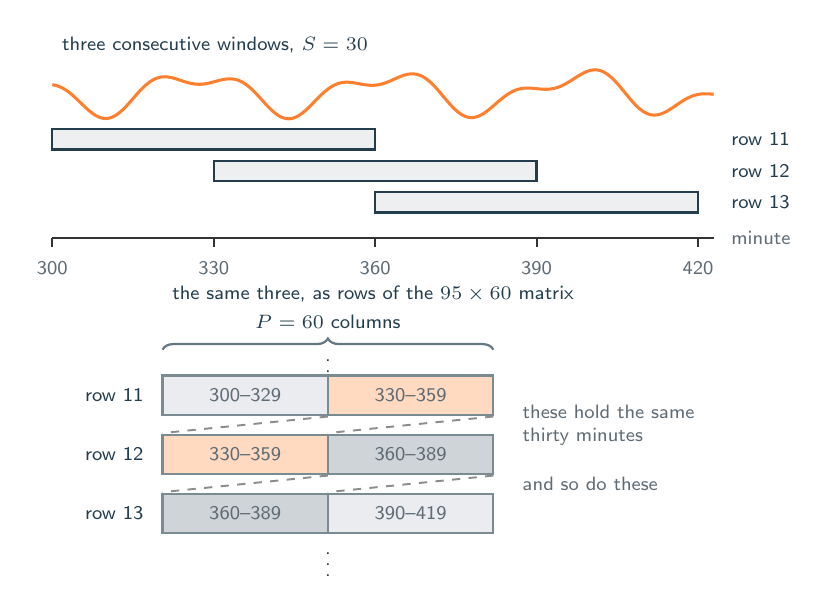
\begin{tikzpicture}[
    every node/.style={font=\sffamily},
    bar/.style={rectangle, draw=c2, fill=c2!8, line width=0.8pt},
    lab/.style={font=\sffamily\scriptsize, text=labelcolor},
    tag/.style={font=\sffamily\scriptsize, text=c2},
    blk/.style={rectangle, draw=c2!60, line width=0.8pt},
    tie/.style={c1!45, line width=0.7pt, dashed},
]

% ============================================================ three windows in time
\node[tag, anchor=west] at (1.20, 7.05) {three consecutive windows, $S = 30$};

\draw[c3, line width=1.1pt]
    plot[domain=1.20:9.60, samples=200, smooth]
    (\x, {6.45 + 0.22*sin(\x r * 2.6) + 0.12*sin(\x r * 5.5 + 30)});

\draw[bar] (1.20, 5.72) rectangle (5.30, 5.98);
\node[tag, anchor=west] at (9.70, 5.85) {row 11};
\draw[bar] (3.25, 5.32) rectangle (7.35, 5.58);
\node[tag, anchor=west] at (9.70, 5.45) {row 12};
\draw[bar] (5.30, 4.92) rectangle (9.40, 5.18);
\node[tag, anchor=west] at (9.70, 5.05) {row 13};

% time axis
\draw[axiscolor, line width=0.8pt] (1.20, 4.60) -- (9.60, 4.60);
\foreach \x/\t in {1.20/300, 3.25/330, 5.30/360, 7.35/390, 9.40/420}{
    \draw[axiscolor, line width=0.7pt] (\x, 4.60) -- (\x, 4.48);
    \node[lab, anchor=north] at (\x, 4.42) {\t};
}
\node[lab, anchor=west] at (9.70, 4.60) {minute};

% ============================================================ the same three, as matrix rows
\node[tag, anchor=west] at (2.60, 3.88)
    {the same three, as rows of the $95 \times 60$ matrix};

\draw[decorate, decoration={brace, amplitude=4pt}, c2!70, line width=0.8pt]
    (2.60, 3.18) -- (6.80, 3.18)
    node[midway, above=4pt, font=\sffamily\scriptsize, text=c2] {$P = 60$ columns};

\node[tag] at (4.70, 3.00) {$\vdots$};

% row 11
\filldraw[blk, fill=c4]    (2.60, 2.35) rectangle (4.70, 2.85);
\filldraw[blk, fill=c3!30] (4.70, 2.35) rectangle (6.80, 2.85);
\node[lab] at (3.65, 2.60) {300--329};
\node[lab] at (5.75, 2.60) {330--359};
\node[tag, anchor=east] at (2.48, 2.60) {row 11};

% row 12
\filldraw[blk, fill=c3!30] (2.60, 1.60) rectangle (4.70, 2.10);
\filldraw[blk, fill=c2!22] (4.70, 1.60) rectangle (6.80, 2.10);
\node[lab] at (3.65, 1.85) {330--359};
\node[lab] at (5.75, 1.85) {360--389};
\node[tag, anchor=east] at (2.48, 1.85) {row 12};

% row 13
\filldraw[blk, fill=c2!22] (2.60, 0.85) rectangle (4.70, 1.35);
\filldraw[blk, fill=c4]    (4.70, 0.85) rectangle (6.80, 1.35);
\node[lab] at (3.65, 1.10) {360--389};
\node[lab] at (5.75, 1.10) {390--419};
\node[tag, anchor=east] at (2.48, 1.10) {row 13};

\node[tag] at (4.70, 0.55) {$\vdots$};

% the shared halves, tied together
\draw[tie] (4.70, 2.33) -- (2.60, 2.12);
\draw[tie] (6.80, 2.33) -- (4.70, 2.12);
\draw[tie] (4.70, 1.58) -- (2.60, 1.37);
\draw[tie] (6.80, 1.58) -- (4.70, 1.37);

\node[lab, anchor=west, align=left] at (7.05, 2.22)
    {these hold the same\\ thirty minutes};
\node[lab, anchor=west, align=left] at (7.05, 1.47)
    {and so do these};

\end{tikzpicture}
\end{document}
